\chapter{EVALUACIÓN DE RIESGOS\label{sec:disenho}}

\clearpage

El objetivo principal que busca la ingeniería de software es convertir el desarrollo de software en un proceso formalizado, con resultados predecibles, que permitan obtener un producto final de alta calidad y satisfaga las necesidades y expectativas del cliente.

Por esta razón, una fase importante es la representación simplificada del proceso para el desarrollo y evaluación de la solución software de este proyecto, desde una perspectiva que señala los beneficios y riesgos de las decisiones que tomamos en los diferentes marcos de trabajo.

Como en un modelo de desarrollo de software, este capítulo rescata etapas como la especificación de requisitos, el diseño, la implementación y la evaluación, teniendo en cuenta los objetivos principales de este proyecto.

\begin{figure}[htp!]
  \centering
  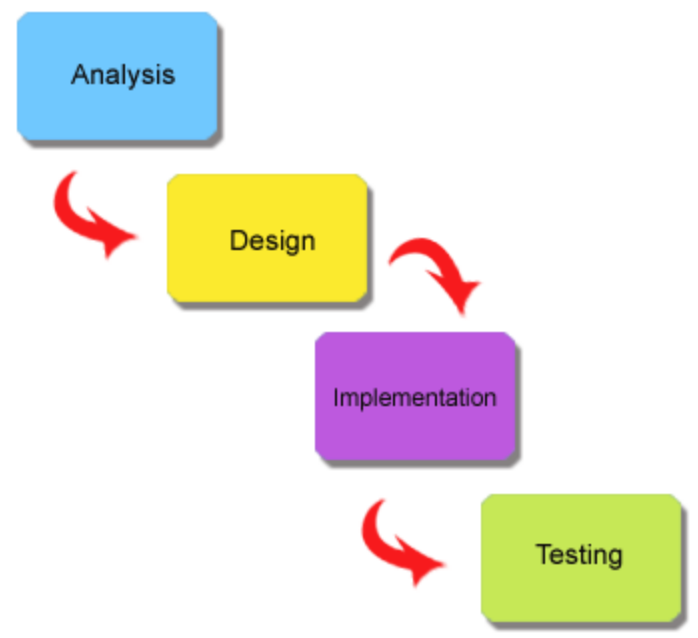
\includegraphics[scale=0.2,clip=true]{waterfall_model}
  \caption{Modelo de desarrollo de software}
  \label{fig:waterfall_model}
\end{figure}

\section{Identificación de los requisitos}

Los requisitos no funcionales tienden a ser aquellos que reflejan la calidad del producto. Especifican los criterios que pueden usarse para juzgar el funcionamiento de un sistema como por ejemplo la disponibilidad, accesibilidad, usabilidad, mantenibilidad, seguridad o rendimiento.

\subsection{Mensajería instantánea}

En la actualidad la mensajería instantánea cada vez tiene una mayor presencia en las empresas. Esta situación hace necesaria la adopción de una serie de requisitos a la hora de autorizar el uso de estos servicios. A continuación se detallan algunos de éstos requisitos:

\begin{itemize}
  \item Confidencialidad de la comunicación. Los mensajes transmitidos a través del servicio de mensajería instantánea sólo pueden ser leídos por el receptor, estableciendo las medidas de seguridad que sean necesarias para evitar que terceros puedan acceder a su contenido.
  \item Integridad del mensaje. Los mensajes no deben poder ser alterados.
  \item Identificación. Los mensajes deben contener la información de su emisor y la persona a la que va dirigido, evitando que el mensaje sea entregado a un destinatario equivocado.
  \item El emisor no debe poder modificar ni eliminar un mensaje ya enviado.
\end{itemize}

\subsection{Centro 112 de Madrid}

A día de hoy, el Centro 112 de Madrid, está consagrado como una gran central de gestión de emergencias que ofrece confianza y seguridad a los ciudadanos. Por lo que nos puede servir como punta de partida en la identificación de los requisitos no funcionales.

Los aspectos más destacados del Centro 112 de Madrid son:

\begin{itemize}
  \item Funciona 24 horas al día y 365 días al año.
  \item Cuenta con 241 profesionales, a los que se suman otros 200 de otros cuerpos y servicios de emergencias que también tienen presencia en el mismo centro de operaciones.
  \item Atiende más de 4,5 millones de llamadas al año, según las últimas publicaciones, y el tiempo medio de respuesta, desde que se establece la llamada al 112 y el operador responde, es de tan solo 8 segundos. Y, que en 70 segundos, el operador ha enviado la emergencia al servicio correspondiente.
  \item La sala de equipos está equipada con herramientas de integración de la telefonía en los puestos de trabajo (PCs), para facilitar el trabajo al operador de emergencias mediante el uso exclusivo de pantalla, teclado y ratón.
  \item Tiene incorporado en su Sistema Integrado de Gestión de Emergencias (SIGE112) la app My112, permitiendo la localización del llamante mediante las coordenadas desde donde se está realizando la llamada.
  \item Su modelo 112 está diseñado con criterios de escalabilidad.
\end{itemize}

Teniendo en cuenta esta información relevante, podemos definir los siguientes requisitos no funcionales que la solución software debe cumplir en todo momento:

\begin{itemize}
  \item Funcionamiento: durante 24 horas seguidas.
  \item Participantes en la comunicación: entre dos o más personas.
  \item Tiempo medio de respuesta: 8 segundos.
  \item Duración media de la comunicación: 70 segundos.
  \item Comunicaciones simultáneas: alrededor de 250.
\end{itemize}

\section{Diseño del protocolo de mensajería instantánea}

Desde hace tiempo se sabe que XML es un formato obsoleto y fallido para la serialización de datos intercambiables. Aunque, proporciona todas las características que XMPP necesita, XML no deja de tener su parte de detractores. De hecho, hace algunos años, esto llevó al intento de proporcionar una codificación binaria para XMPP llamada Binary XMPP.

Desafortunadamente, la codificación binaria carecía de las principales ventajas de XML en su legibilidad humana, por lo que la búsqueda de mejores codificaciones nos lleva a JSON.

Por otro lado, si en nuestro proyecto no fuese crítico la comunicación inmediata, sería una buena idea respaldarse en la simplicidad del long pooling. Algunos desarrolladores prefieren usar long pooling porque las tecnologías modernas como son los WebSockets son más complejas y difíciles de configurar. Cuando la simplicidad no es tan importante como el rendimiento, hay que considerar el uso de WebSockets.

\subsection{Mensajería instantánea grupal}

Hoy en día, hay aplicaciones para casi cualquier cosa, incluidas aplicaciones como WhatsApp que te permiten conectarte con dos o más personas al mismo tiempo. Una de las características destacadas de estas aplicaciones de mensajería instantánea es que permiten que grupos grandes hablen y conversen al mismo tiempo. Conocidas como mensajería instantánea grupal, estas aplicaciones las ofrecen de forma predeterminada sin costo.

Dada la naturaleza competitiva de la industria, hay varias aplicaciones que realizan una función similar. Con la multitud de aplicaciones que existen, puede ser bastante difícil elegir una aplicación como base para nuestro desarrollo. Teniendo esto en cuenta, es esencial que nuestra aplicación permita como mínimo el envío de mensajes de texto en un grupo.

\subsection{WebSocket}

Como se ha visto, WebSocket permite establecer comunicaciones bidireccionales en tiempo real en la Web, posibilidad que antes solo existía de forma simulada y bastante costosa mediante técnicas como long polling.

Optar por WebSocket permite reducir la saturación de cabeceras que ocurriría si se utilizase HTTP en su lugar, especialmente para aplicaciones web que requieren un gran volumen de comunicaciones. Además, evita que cada aplicación web utilice una solución de integración diferente, con los problemas de compatibilidad que ello conlleva.

También, se ha visto que su funcionamiento es extremadamente sencillo: se establece una conexión, se envían/reciben mensajes y se cierra la conexión. Al funcionar bajo los mismos puertos que HTTP evita problemas relacionados con cortafuegos, facilitando así el funcionamiento de productos basados en SOA, entre otros.

Por otra parte, es necesario gestionar y mantener un gran número de conexiones que han de permanecer abiertas mientras ambas partes sigan interactuando. Esto puede llegar a ser un problema en determinados casos, teniendo en cuenta que el número máximo de conexiones simultáneas que admite un puerto TCP es de 64.000 y que, además, mantener las conexiones abiertas requiere memoria del servidor.

Por tanto, WebSocket es la mejor solución para aplicaciones web que necesitan actualizaciones constantes en tiempo real como chats, juegos multijugador en línea o retransmisiones interactivas en directo.

\subsection{JSON}

Originalmente, el lenguaje XML era increíblemente flexible y fácil de escribir, pero su inconveniente era que era detallado, difícil de leer para los humanos, muy difícil de leer para los servidores, y tenía mucha sintaxis que no era del todo necesaria para comunicar información.

Hoy en día, XML está muerto para la serialización de datos en la web. A menos que esté escrito en HTML o SVG, ambos hermanos en XML, probablemente no verás XML en otros lugares. Algunos sistemas obsoletos todavía lo usan hoy, pero usarlo para pasar datos tiende a ser excesivo para la web.

La transferencia de datos es mucho más fácil cuando los datos se almacenan en una estructura que está familiarizada a los lenguajes orientados a objetos por lo que es muy sencillo importar datos desde un fichero JSON a Perl, Ruby, JavaScript, Python, y otros muchos lenguajes. En XML, tendríamos que transformar los datos antes de importarlos. Por esta razón, JSON es un formato de fichero superior para las Web APIs.

JSON se usa en todas partes hoy en día. El formato es fácil de escribir tanto por humanos como por máquinas, y se convirtió en el estándar de facto para transferir datos de un sistema a otro. Casi todos los lenguajes de programación tienen una funcionalidad incorporada para leerlos y escribirlos.

Otra de las grandes ventajas que presenta JSON es el rendimiento, ya que los JSON son considerablemente más livianos en peso y mucho más rápido en su procesamiento. Pero como ya vimos, el rendimiento tiene un coste y es la robustez del mensaje como tal.

Un objeto JSON es un objeto válido en JavaScript por lo que es el formato perfecto para este lenguaje. La mayoría de los navegadores web modernos incluyen funciones nativas para codificar y decodificar JSON, lo que le da un punto de ventaja en lo que se refiere a desempeño y disminuyen los riesgos de seguridad.

\section{Desarrollo de la aplicación web en tiempo real}

Una aplicación web en tiempo real requiere un esfuerzo de ingeniería muy grande. En un modelo tradicional son los clientes los que preguntan al servidor, lo que requiere poco trabajo por parte de éste. Las peticiones llegan y el servidor responde. Fácil y sencillo. El servidor no procesa más datos de los necesarios para dar la información que piden los clientes.

Cuando pasamos al modelo del tiempo real, las cosas cambian. Ahora el servidor tiene que preocuparse de dar la información a los clientes cuando ésta se genera. Para ello necesita un registro de clientes que tienen que recibir esa información, así que no sólo tiene que procesar los datos relativos a la información que va a dar sino que además tiene que preocuparse de decidir con quién conectar y cuándo hacerlo. No sólo eso, también tiene que gestionar las conexiones y desconexiones del sistema. Es decir, un método mucho más complejo que el tradicional.

Con toda esa complejidad del tiempo real, alguna ventaja tenía que darnos. La primera es para los servidores. En una aplicación web tradicional, por ejemplo, si de repente los 200.000 clientes de un servicio deciden hacer una petición todos a la vez, el servidor puede bloquearse por saturación. Sin embargo, si son los servidores los que gestionan las conexiones estas situaciones no pueden ocurrir: el servidor distribuye de forma normal las conexiones de forma que no haya problemas de saturación, y evitando los ataques DDoS involuntarios.

La siguiente ventaja es bastante obvia: la instantaneidad de la información. Cuando son las aplicaciones las que tienen que preguntar al servidor, normalmente lo hacen a intervalos usando pooling. Si vamos encadenando varias aplicaciones, los intervalos se acumulan y podemos tener retardos bastante grandes. Con una aplicación web en tiempo real, estos intervalos desaparecen y la información llega con un retraso mínimo.

Otra ventaja es que genera menos tráfico de red. Por ejemplo, si un cliente de correo comprueba cada cinco minutos si tiene mensajes nuevos, cada cinco minutos va a estar generando tráfico haya o no haya mensajes nuevos. Es decir, que estará creando bastante tráfico inútil. Sin embargo, si es el servidor el que avisa al cliente, sólo se produce tráfico cuando hay correo nuevo. De este modo, el tráfico generado es siempre tráfico útil.

\subsection{REST}

REST es una tecnología que transporta datos por medio del protocolo HTTP. Es tan flexible que permite transmitir prácticamente cualquier tipo de datos, ya que el tipo de datos está definido por la cabecera Content-Type, lo que nos permite mandar formatos como XML o JSON, binarios (imágenes, documentos), texto plano, entre otros más.

\begin{figure}[htp!]
  \centering
  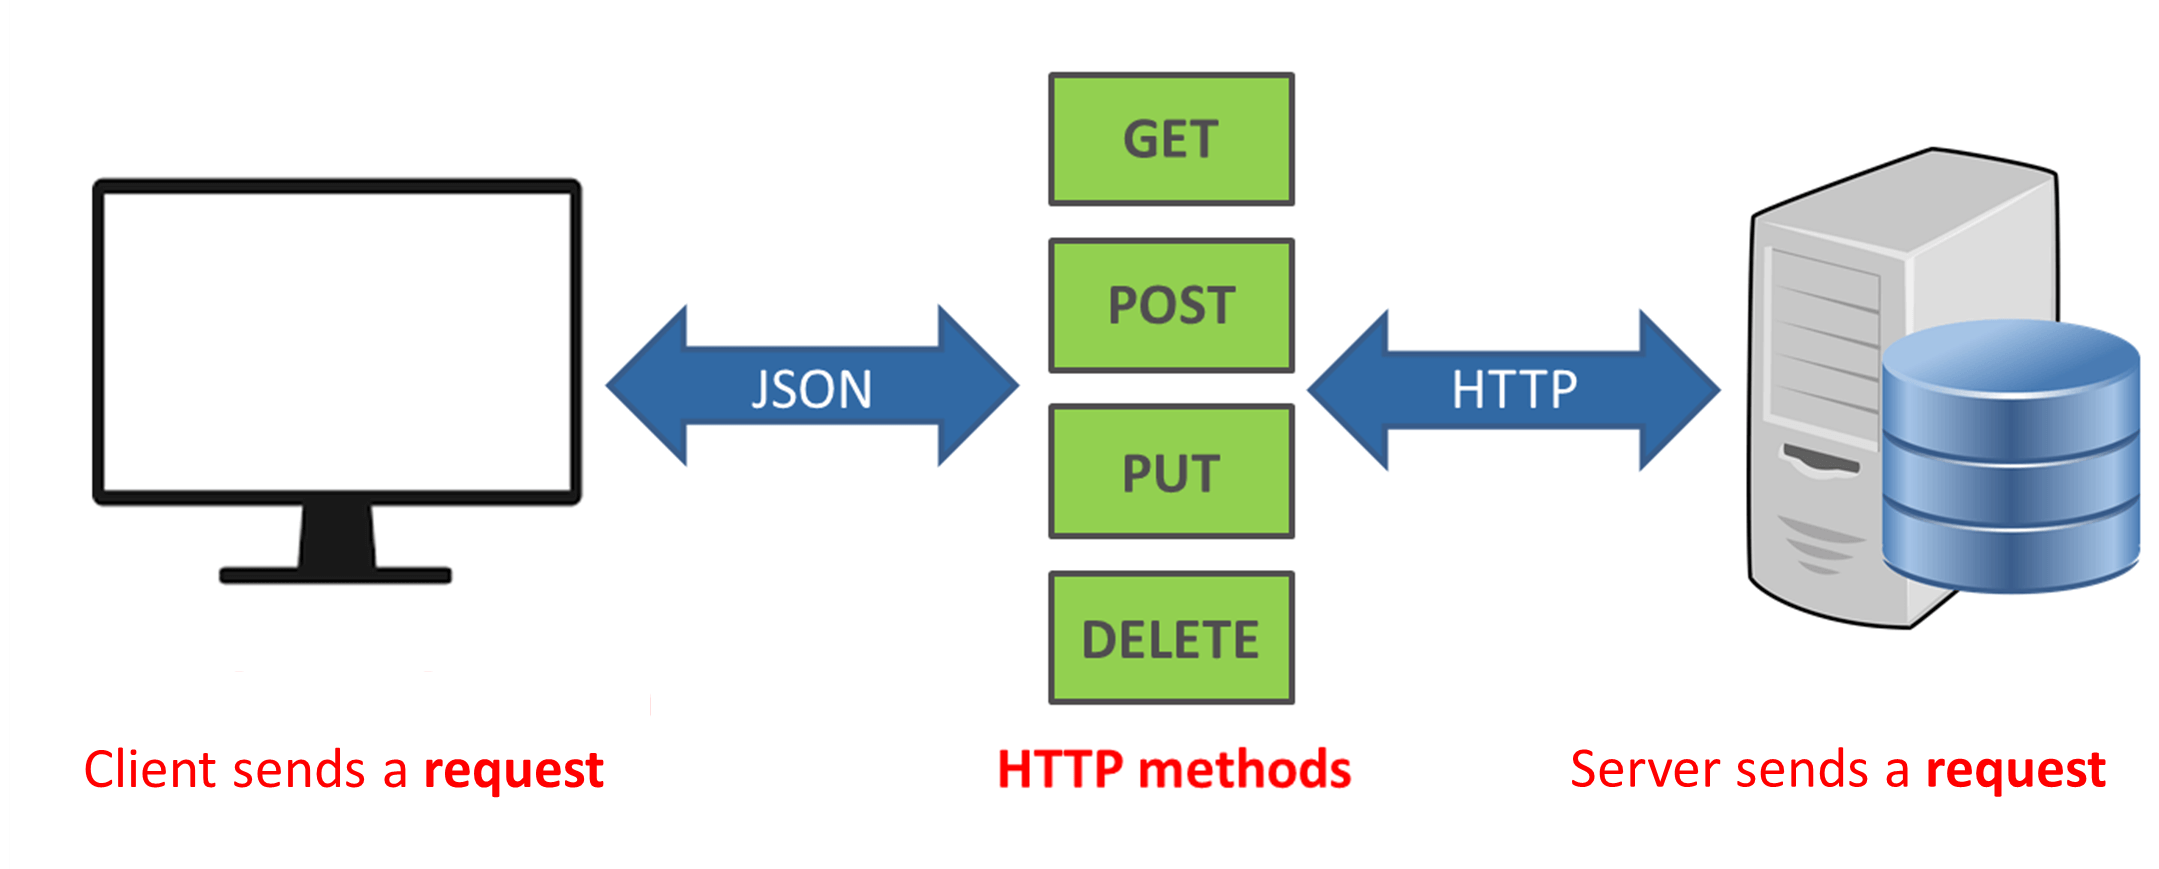
\includegraphics[scale=0.1,clip=true]{rest}
  \caption{Arquitectura de REST}
  \label{fig:rest}
\end{figure}

REST se caracteriza por no tener estado. Es decir, el servidor no es capaz de recordar el estado de la anterior solicitud REST que pudo, o no, hacer un cliente. Por ello, el cliente tiene que enviar en cada solicitud todo el estado de su sesión.

REST viene para simplificar las cosas. Hoy REST y JSON se han convertido en la opción más sencilla y por tanto más recomendable para implementar una aplicación web.

\subsection{Node.js}

Gracias a que Node.js permite trabajar tanto desde el servidor como desde el cliente, es posible generar una transferencia de información mucho más rápida e inmediata. El resultado de todo esto es una reducción considerable en los periodos de trabajo.

Además al ser un lenguaje popular y empleado por profesionales de todo el mundo resulta fácil encontrar información y recursos en Internet. Está diseñado para incentivar el intercambio entre usuarios y programadores.

Es quizá la opción más competitiva para diseñar aplicaciones que gestionan grandes cantidades de información generadas por una comunidad elevada de usuarios.

Debido a sus altas prestaciones para gestionar y procesar grandes volúmenes simultáneos de información, Node.js es una opción estrella para el desarrollo de aplicaciones como chats online.

\subsubsection{Beneficios de utilizar Node.js}

Asumiendo que lo que interesa son las ventajas desde el punto de vista del desarrollo web, a continuación se definen las más significativas:

\begin{itemize}
  \item Escalabilidad de manera sencilla. Node.js se diseñó con una arquitectura dirigida por eventos y con E/S asíncrona desde el minuto 0. Eso hace que sea muy escalable de forma sencilla y directa.
  \item Rendimiento. Gracias al motor V8 el uso de Javascript en Node.js supera a soluciones basadas en otros lenguajes “interpretados”.
  \item Javascript. Node.js está basado en Javascript, que es un lenguaje que está de moda, en parte gracias al propio Node.js. Y además es el lenguaje de la web. El único soportado por todos los navegadores. Ahora que las aplicaciones web se han hecho muy interactivas y que es ingente la cantidad de código en Javascript que corre en los navegadores, es muy cómodo poder desarrollar con el mismo lenguaje en el servidor.
  \item Popularidad. Como he mencionado todo esto ha llevado a que Node.js y Javascript gocen de gran popularidad. Cada vez hay más interés y más desarrolladores. Y eso hace que la comunidad sea enorme, lo que es muy interesante en caso de necesitar ayuda.
\end{itemize}

\subsubsection{Event Loop de Node.js}

Si una empresa desea que su aplicación soporte más usuarios, necesitará agregar más y más servidores. Por todas estas razones, el cuello de botella en toda arquitectura de aplicaciones web es el número máximo de conexiones concurrentes que podía manejar un servidor.

Node.js resuelve este problema cambiando la forma en que se realiza una conexión con el servidor. En lugar de generar un nuevo hilo del sistema operativo para cada conexión (y de asignarle la memoria acompañante), cada conexión dispara una ejecución de evento dentro del proceso del motor V8 de Node.js.

Node.js emplea un único hilo y un event loop asíncrono. Las nuevas peticiones son tratadas como eventos en este bucle. Este es el motivo por el que las características asíncronas y los eventos de JavaScript encajan tan bien en la filosofía de Node.js.

\begin{figure}[htp!]
  \centering
  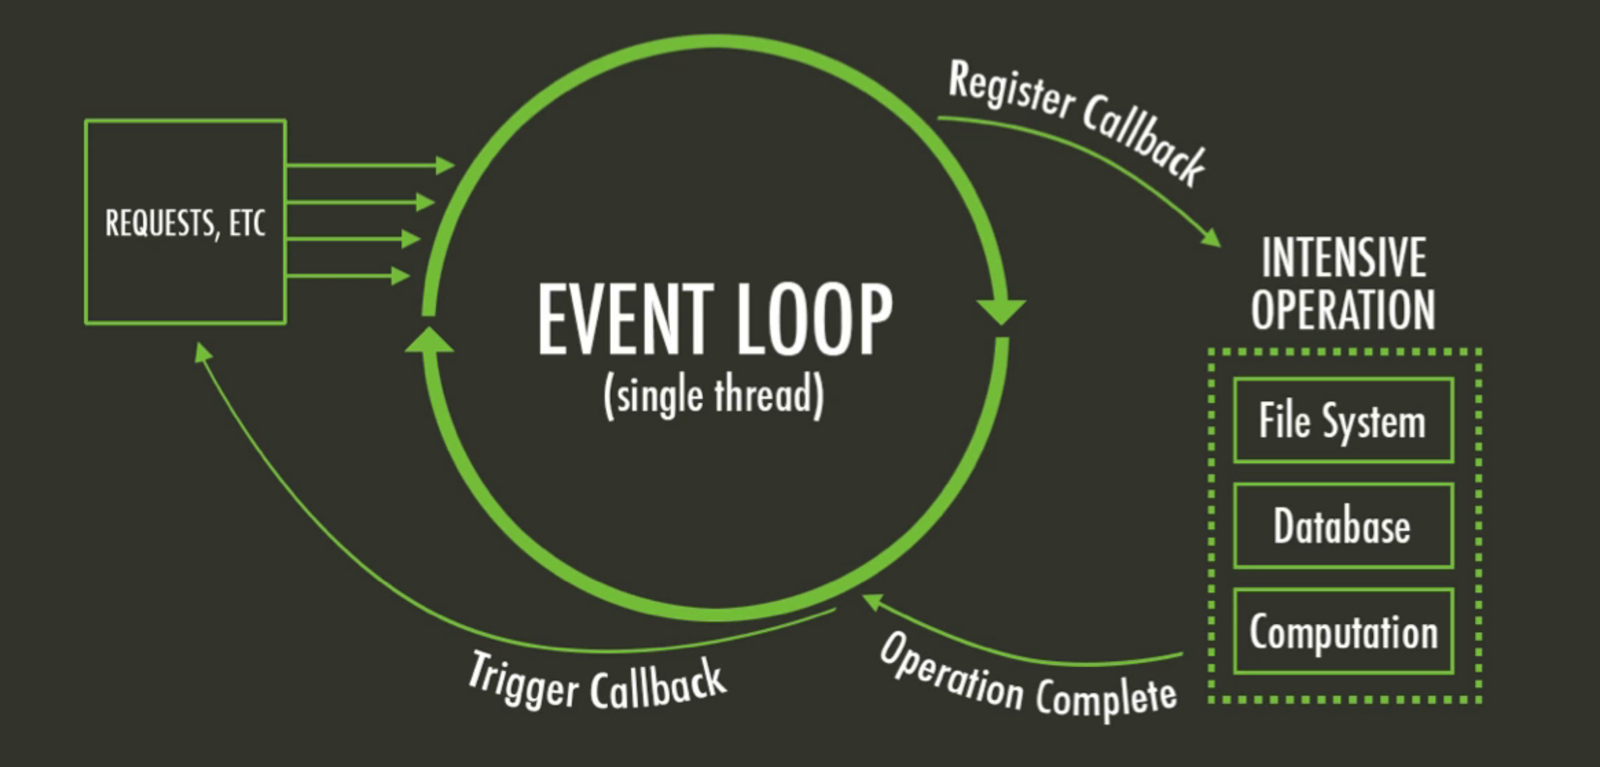
\includegraphics[scale=0.2,clip=true]{nodejs_eventloop}
  \caption{Event Loop de V8}
  \label{fig:nodejs_eventloop}
\end{figure}

Esto permite que Node.js sea capaz de gestionar múltiples conexiones y peticiones de forma muy eficiente, lo que lo hace apropiado para desarrollo y aplicaciones con un gran número de conexiones simultáneas.

\subsubsection{NPM}

En un proyecto Node.js, el código se organiza por módulos o paquetes, así que al momento de trabajar con él va a ser necesario agregar más módulos, es aquí donde entra la herramienta NPM.

\begin{figure}[htp!]
  \centering
  
\includegraphics[scale=0.05,clip=true]{npm_logo}
  \caption{Logo de NPM}
  \label{fig:npm_logo}
\end{figure}

Node Package Manager, o simplemente npm, es un gestor de paquetes, el cual hará más fácil nuestras vidas al momento de trabajar con Node.js, ya que gracias a él podremos tener cualquier librería disponible con solo una línea de código. NPM nos ayudará a administrar nuestros módulos, distribuir paquetes y agregar dependencias de una manera sencilla.

\subsubsection{Express.js}

Muchos desarrolladores de software han optado por utilizar JavaScript para construir aplicaciones web. Esto ha provocado un crecimiento exponencial de los frameworks web para Node.js con el objetivo de facilitar la creación rápida de prototipos y la construcción de aplicaciones web impresionantes, especialmente en el lado del servidor.

Los frameworks para Node.js se utilizan principalmente debido a su productividad, escalabilidad y velocidad, lo que los convierte en una de las primeras opciones para crear aplicaciones web para empresas.

Al usar un framework, puedes trabajar con un conjunto de herramientas, directrices y prácticas recomendadas que lo ayudan a ahorrar tiempo. También puede ayudar a consolidar los estándares de código en un equipo de desarrolladores.

Express.js es un framework web rápido, flexible y minimalista para Node.js. Es simplemente una tecnología basada en Node.js que se comporta como un middleware para ayudar a administrar nuestros servicios y rutas.

\begin{figure}[htp!]
  \centering
  
\includegraphics[scale=0.2,clip=true]{express_logo}
  \caption{Logo de Express.js}
  \label{fig:express_logo}
\end{figure}

Express.js ha demostrado, con el tiempo, que su popularidad vale la pena con sus métodos y funciones fáciles de usar. Probablemente sea el framework web para Node.js más popular disponible para la comunidad de JavaScript en GitHub con más de 41,000 estrellas.

Algunas de las numerosas ventajas de Express.js incluyen:

\begin{itemize}
  \item Casi el estándar para el middleware web de Node.js.
  \item Totalmente personalizable.
  \item Curva de aprendizaje baja.
\end{itemize}

\subsection{MongoDB}

Es muy común entre los desarrolladores de aplicaciones web encontrarse en la situación de tener que elegir si se va a usar una base de datos SQL o NoSQL. La mayoría no se lo piensa demasiado y opta por la opción que mejor conocen y con la que más cómodos trabajan. Tampoco es una decisión catastrófica; en realidad, ya sea una base de datos SQL o NoSQL, se puede construir cualquier cosa.

Es importante saber en qué se diferencian y cuál deberíamos usar en cada caso, ya que un buen diseño de base de datos con la tecnología apropiada indudablemente aporta calidad al proyecto. Dependiendo de la naturaleza de la aplicación, interesa que la base de datos tenga unas características u otras.

La diferencia fundamental entre ambos tipos de base de datos radica en que las bases de datos NoSQL no hacen uso de un modelo relacional. Si tu proyecto necesita una escalabilidad importante, donde los recursos son escasos y no necesita respetar la integridad de los datos, entonces sí: NoSQL es la mejor opción.

A la hora de hacer una aplicación web, existen varias soluciones para cada uno de los grandes componentes que forman una aplicación completa. Si el servidor web está en Node.js, MongoDB es la base de datos NoSQL que tiene más éxito entre este tipo de aplicaciones.

\begin{figure}[htp!]
  \centering
  
\includegraphics[scale=0.1,clip=true]{mongodb_logo}
  \caption{Logo de MongoDB}
  \label{fig:mongodb_logo}
\end{figure}

\subsubsection{Beneficios de MongoDB}

Los siguientes son algunos de los beneficios y fortalezas de MongoDB:

\begin{itemize}
  \item Esquema dinámico. como se mencionó, esto le brinda flexibilidad para el esquema de los datos sin modificar ninguno de los datos ya existentes.
  \item Escabilidad. MongoDB es escalable horizontalmente, lo que ayuda a reducir la carga de trabajo y la escala de tu negocio con facilidad.
  \item Capacidad de administración. la base de datos no requiere un administrador de base de datos. Ya que es bastante fácil de usar de esta manera, puede ser utilizado tanto por desarrolladores como por administradores.
  \item Velocidad. Es de alto rendimiento para consultas simples.
  \item Flexibilidad. puede agregar nuevas columnas o campos en MongoDB sin afectar las filas existentes o el rendimiento de la aplicación.
\end{itemize}

\subsection{Docker}

Aunque, por su naturaleza, se asemejan a las clásicas máquinas virtuales, estamos hablando de algo más avanzado porque nos ofrecen una mayor eficiencia y sencillez.

Para empezar, los contenedores de Docker comparten recursos con el sistema operativo sobre el que se ejecutan. De esta manera podemos arrancar o parar el contenedor rápidamente, mientras que las máquinas virtuales se aíslan del sistema operativo sobre el que trabajan y se comunican a través del hypervisor \cite{docker2}.

La portabilidad de los contenedores hace que los problemas causados por cambiar el entorno donde está corriendo la aplicación se reduzcan a la mínima expresión.

En cuanto al rendimiento, existen diferencias respecto a una virtualización de máquina completa. Los tiempos de arranque son menores. Además, el nivel de aislamiento es menor y ciertas partes de la memoria del contenedor están duplicadas, lo que permite ejecutar múltiples instancias del mismo contenedor sin que ello suponga una gran merma de la memoria.

\subsubsection{Ventajas de los contenedores de Docker}

Las ventajas de los contenedores Docker son:

\begin{itemize}
  \item Modularidad. El enfoque Docker para la creación de contenedores se centra en la capacidad de tomar una parte de una aplicación, para actualizarla o repararla, sin necesidad de tomar la aplicación completa.
  \item Control de versiones de imágenes y capas. Cada archivo de imagen de Docker se compone de una serie de capas. Estas capas se combinan en una sola imagen. Una capa se crea cuando la imagen cambia. Docker reutiliza estas capas para construir nuevos contenedores, lo cual hace mucho más rápido el proceso de construcción.
  \item Restauración. Probablemente la mejor parte de la creación de capas es la capacidad de restaurar. Si no te gusta la iteración actual de una imagen, restaura la versión anterior.
  \item Implementación rápida. Solía demorar días desarrollar un nuevo hardware, ejecutarlo, proveerlo y facilitarlo. Y el nivel de esfuerzo y sobrecarga era extenuante. Los contenedores basados en Docker pueden reducir el tiempo de implementación a segundos.
\end{itemize}

\section{Diseño del entorno de pruebas}

Una vez que tengamos probada y desplegada nuestra aplicación, se debe probar de forma automática las capacidades y debilidades del software y de la plataforma sobre la que está corriendo (infraestructura y dependencias), llevándola al límite, para comprobar su disponibilidad, estabilidad y resiliencia.

\subsection{Pruebas no funcionales}

Las pruebas no funcionales se refieren a aspectos del software que pueden no estar relacionados con una función específica o acción del usuario, como la escalabilidad o el comportamiento bajo ciertas restricciones o la seguridad. Estas pruebas determinan el punto de ruptura, el punto en el que los extremos de escalabilidad o rendimiento llevan a una ejecución inestable.

Podemos clasificar las pruebas no funcionales según el tipo de requisito no funcional que abarcan:

\subsubsection{Pruebas de seguridad}

Las pruebas de seguridad validan los servicios de seguridad de una aplicación e identifican posibles fallos y debilidades. Las pruebas de seguridad son esenciales para el software que procesa datos confidenciales para evitar la intrusión en el sistema por parte de hackers informáticos.

Muchos proyectos utilizan un enfoque de caja negra para las pruebas de seguridad, lo que permite a los expertos, sin conocimiento del software, probar la aplicación en busca de agujeros, fallos, exploits y debilidades.

\subsubsection{Pruebas de usabilidad}

Las pruebas de usabilidad son para verificar si la interfaz de usuario es fácil de usar y entender. Se refiere principalmente a la interacción con la aplicación. Este no es un tipo de prueba que se pueda automatizar; se necesitan usuarios reales, que sean monitoreados por diseñadores de interfaces de usuario expertos.

\subsubsection{Pruebas de rendimiento}

Las pruebas de rendimiento verifican la capacidad de respuesta, el rendimiento, la confiabilidad y/o la escalabilidad del sistema cuando está bajo una carga de trabajo significativa.

Por su naturaleza, las pruebas de rendimiento pueden ser bastante costosas de implementar y ejecutar, pero pueden ayudarte a entender si los nuevos cambios van a degradar o mejorar el rendimiento del sistema.

En aplicaciones web, las pruebas de rendimiento a menudo están estrechamente relacionadas con las pruebas de estrés, la medición del retraso y la capacidad de respuesta bajo una carga pesada. Por ejemplo, se pueden observar los tiempos de respuesta cuando se ejecuta una gran cantidad de peticiones de usuario, o ver cómo se comporta el sistema con una cantidad significativa de datos.

\subsection{Diseño de pruebas de rendimiento}

Las pruebas de rendimiento generalmente se ejecutan para determinar cómo se desempeña un sistema o subsistema en términos de capacidad de respuesta y estabilidad bajo una carga de trabajo en particular. Pero, también puede servir para investigar, medir, validar o verificar otros atributos de calidad del sistema, como la escalabilidad, la confiabilidad y el uso de recursos.

\subsubsection{Pruebas de carga}

Las pruebas de carga se encarga principalmente de comprobar que el sistema puede continuar operando bajo una carga de trabajo específica, ya sea en grandes cantidades de datos o en una gran cantidad de peticiones. Esta carga puede ser el número esperado de usuarios concurrentes, que utilizando la aplicación realizan un número específico de transacciones durante el tiempo que dura la carga.

Una prueba de carga puede mostrar los tiempos de respuesta de todas las transacciones importantes de la aplicación. Esto generalmente se conoce como escalabilidad de software.

Si también se monitorizan otros aspectos como la base de datos, el servidor de aplicaciones, etcétera, entonces esta prueba puede mostrar el cuello de botella de la aplicación.

\subsubsection{Pruebas de estrés}

La prueba de estrés empuja los límites funcionales de un sistema. Se realiza sometiendo el sistema a condiciones extremas, como volúmenes de datos máximos o una gran cantidad de usuarios simultáneos. Se utiliza normalmente para romper la aplicación.

Se va doblando el número de usuarios que se agregan a la aplicación y se ejecuta una prueba de carga hasta que se rompe. Esto ayuda a los administradores para determinar si la aplicación rendirá lo suficiente en caso de que la carga real supere a la carga esperada.

También se utilizan para, llevado el sistema al colapso o degradación, comprobar su funcionamiento continuado por encima de su límite y, una vez liberado de la carga, evaluar su capacidad de resiliencia volviendo a su estado óptimo de funcionamiento.

\subsubsection{Pruebas de estabilidad}

Las pruebas de estabilidad o soak testing comprueban si el software puede funcionar continuamente en un período aceptable o superior; es decir, si la aplicación puede aguantar una carga esperada continuada. Generalmente esta prueba se realiza para determinar si hay alguna pérdida de memoria (memory leak) en la aplicación.

Las pruebas de estabilidad son una gran prueba, que a menudo se pasa por alto, y que muestra muchos aspectos críticos sobre una aplicación bajo carga de trabajo constante, cosas que ninguna otra prueba puede y es crítica para determinar si la aplicación es apta para la producción.

Hay que tener en cuenta los requisitos de la aplicación, la organización y la producción para determinar el largo periodo de tiempo que la prueba de estabilidad estará ejecutándose.

En una organización en la que los sistemas de producción se apagan y reinician todas las noches, la prueba de estabilidad no debe durar más de 24 horas. En cambio, si la aplicación se reinicia semanalmente como parte de un ciclo de mantenimiento, entonces la prueba de estabilidad debe durar al menos 7 días.

\subsection{Herramienta para pruebas de rendimiento}

Existen numerosas herramientas, tanto open source como privadas, para realizar las pruebas de rendimiento: NeoLoad, LoadRunner, LoadUI, WebLOAD, Artillery, etcétera. Una de las más populares es Apache JMeter.

Apache JMeter es una herramienta para llevar a cabo simulaciones sobre cualquier recurso de software. Es una herramienta creada por Apache y está completamente escrita en Java.

\begin{figure}[htp!]
  \centering
  
\includegraphics[scale=0.3,clip=true]{jmeter_logo}
  \caption{Logo de Apache JMeter}
  \label{fig:jmeter_logo}
\end{figure}

Apache Jmeter se suele usar para hacer pruebas de carga aunque también soporta aserciones para asegurar que los datos recibidos son correctos y muchas posibilidades a la hora de generar reportes.

\subsubsection{Java}

TODO
